\documentclass[10pt,a4paper]{report}
\usepackage[utf8x]{inputenc}
\usepackage[english]{babel}
\usepackage{amsmath}
\usepackage{amsfonts}
\usepackage{amssymb}
\usepackage{makeidx}
\usepackage{fancyhdr}
\usepackage{fancybox}
\usepackage{geometry}
\usepackage{graphicx}
\usepackage{caption}
\usepackage{subcaption}


\author{Robert Michit - Maurin Nadal - Laurent Dutertre}
\title{Triades - User manual}

\newcommand{\tria}{\textbf{Triades }}


\geometry{hmargin=2.5cm, vmargin=3cm}



\pagestyle{fancy}
\fancyhf{}

%\renewcommand{\chaptermark}[1]{\markboth{\bsc{\chaptername~\thechapter{} :} #1}{}} 
%\renewcommand{\sectionmark}[1]{\markright{\thesection{} #1}}

\rhead{\tria - version 1.0.3}
\lhead{\leftmark}

%\cfoot{\thepage / \pageref{\LastPage}}
\addtolength{\fboxsep}{10pt}



\begin{document}


% page de garde
\begin{titlepage}
~\\
\vspace{50pt}

\begin{center}

\includegraphics[height = 6cm]{images/splashScreen.png} 


\vspace{230pt}
\begin{Huge}
\tria - User manual\\
\end{Huge}
\begin{Large}
\vspace{20pt}
Version 1.0.1\\

\end{Large}
Robert Michit - Maurin Nadal - Laurent Dutertre
\end{center}

\end{titlepage}



% table des matières

% introduction



\tableofcontents
\chapter*{Introduction}

\tria est un logiciel permettant d'identifier facilement des lieux de problèmes dans des situations relationnelles courantes. Ces situations ont été schématisées au préalable et le but de \tria est de fournir un accès facile et rapide aux informations qui intéressent le plus l'utilisateur.\\

Dans un deuxième temps, \tria permet d'exporter les schémas importants sous la forme d'images afin de les utiliser dans le cadre d'une présentation ou d'un rapport. Il est possible de fortement personnaliser l'apparence des schémas lors de ces exportations pour les adapter au cadre d'utilisation.\\

L'utilisation classique se déroule de la manière suivante :\\
\begin{enumerate}
\item Création d'une session, l'utilisateur choisi dans une liste l'ensemble des acteurs concernés par la situation sur laquelle il veut travailler. Il est possible de saisir les deux récits des différents acteurs lors de cette étape.\\
\item Navigation dans les différentes situations impliquant ces acteurs. Un système de navigation permet a l'utilisateur d'accéder à l'ensemble des briques pouvant l'intéresser (chaque brique correspond à une situation réelle). Un classement permet à l'utilisateur de se concentrer en premier sur les briques qui sont à priori les plus intéressantes.\\
\item L'utilisateur saisi les relations liants les différents acteurs dans chaque situation. Le logiciel met alors en avant les relations en écart avec une situation théorique correcte.\\
\item Une fois ces lieux identifiés, l'utilisateur exporte les schémas concernés vers des images en mettant en valeur les lieux de problèmes. Ces images permettront de faciliter la résolution des problème en accélérant la compréhension des mécanismes sous-jacent.\\
\end{enumerate}



\begin{figure}[h!t]
\centering
\Ovalbox{
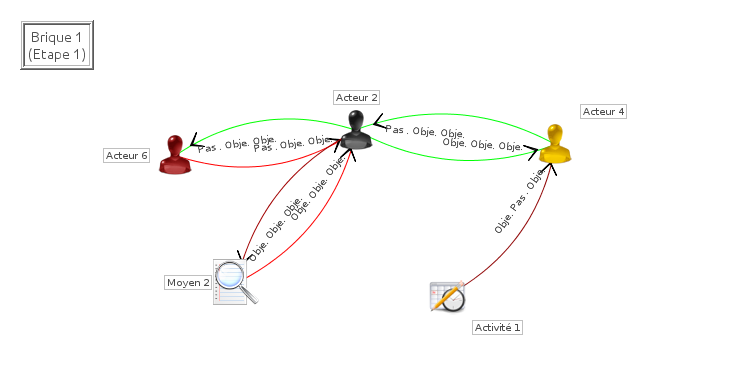
\includegraphics[width=12cm]{images/exportOrigin.png}
}
\caption{Une brique lors de l'édition de ses relations}
\vspace*{15pt}
\Ovalbox{
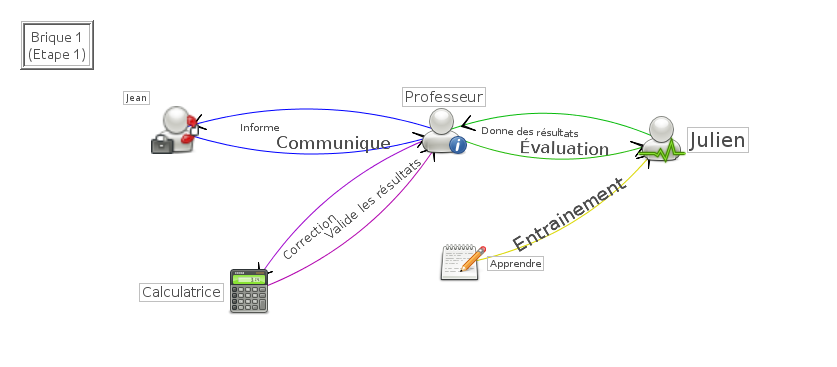
\includegraphics[width=12cm]{images/exportModifie.png}
}
\caption{La même une fois personnalisée afin d'être exportée.}


\end{figure}



\chapter{General information}
\section{Automatic datapack download and update}
During the first launch of student version of \tria, the user have to enter the address to download the datapack. Indeed, the student version installer does not contains a datapack in order to allow a easier distribution of sessions and local datapack translation. It is possible that the software needs to be restarted after the downloading of the datapack file.\\

%Lors du premier lancement de la version étudiante, l'utilisateur est invité à saisir une adresse à laquelle le datapack peut être téléchargé. En effet, le logiciel en version étudiante est initialement fourni sans datapack afin de permettre un déploiement plus aisé de nouvelles sessions ou d'une traduction locale du contenu du datapack. Il est possible qu'il soit nécessaire de relancer le logiciel une fois le fichier téléchargé.\\

\subsection{AutoUpdater software}
The software "AutoUpdater" do an automatic update of the datapack from a file downloaded from internet.\\
%Le programme "AutoUpdater" permet de mettre à jour automatiquement le datapack à partir d'un fichier téléchargé sur internet.\\

When "AutoUpdater" is launched, the user have to input the address where the datapack could be downloaded. When the old datapack and the new one contains a translation or some sessions sharing the same name, the user is asked about which version he wants to keep.\\
%Lors du lancement de l'autoUpdater, l'utilisateur est invité à saisir l'adresse de téléchargement du datapack. Dans le cas où le datapack courant et le nouveau contiennent une traduction ou des sessions portant le même nom, le programme demande à l'utilisateur quelle version il souhaite conserver.\\

A backup of the old datapack is automatically done, the backup file is placed in the sub-folder "datapack\_backup".\\
%Une sauvegarde de l'ancien datapack est automatiquement réalisée et placée dans le dossier "datapack\_backup".

\section{License management}
Datapack used with student version have a limited trial time. When buying a use license, an unlocking code is given. This code could be entered in the software with the option "Register a license" in the "Help menu". A dialog pop-up, to request the mail address associated with the license and the registration code.\\

%Les datapacks fournis avec la version étudiante du logiciel ont un durée d'utilisation limitée dans le temps. Lors de l'achat d'une licence, un code de déblocage du datapack est fourni. Ce code peut être saisi à l'aide de l'option "Enregistrer une licence". Une fenêtre s'ouvre alors invitant l'utilisateur à saisir l'adresse mail associée à la licence puis le code de validation.\\

When the software is launched with an expired datapack, a dialog pop-up to request from the user his license information. The software could need to be restarted after registering a license. 
%Lors de l’utilisation d'un datapack dont la durée d'essai s'est achevé, une boite de dialogue invite l'utilisateur à saisir ces mêmes informations pour permettre l'utilisation du datapack. Il est possible qu'un redémarrage du logiciel soit nécessaire lors de la saisie d'une licence.\\





% 1 Sessions et liste de d'acteurs
% 1.1 Session
% 1.2 Selection des acteurs
% 1.3 fiche acteurs
\chapter{Les sessions}

Chaque session correspond à un cas d'étude différent. Lorsque le logiciel est utilisé pour analyser une situation inédite, une nouvelle session doit être créée.\\

Une session est caractérisée par un ensemble d'acteurs plus ou moins importants (acteurs principaux et secondaires) et par les deux récits associés à chacun de ces acteurs. De plus, l'utilisateur donner un nom spécifique à chaque acteur afin de faciliter la compréhension des briques (ainsi, un acteur "père" peut être renommé en "M. X" au sein d'une session, ce renommage n'aura un impact qu'à l'intérieur de cette session).\\

\section{Choix de la session}
Lors du lancement du logiciel, l'utilisateur est amené à choisir entre 3 options :\\
\begin{enumerate}
\item Editer l'ensemble des schémas : Cela correspond à une session générée automatiquement. Elle correspond à la sélection de tous les acteurs possibles. Cette session permet d'avoir une vue globale des situations schématisées dans le logiciel.
\item Créer une nouvelle session : Lance le processus de création d'une session.
\item Ouvrir une ancienne session : La liste des sessions précédentes se situe juste au dessous de cette option. Un double clique sur la ligne d'une ancienne session permet de l'ouvrir automatiquement.
\end{enumerate}

\begin{figure}[h!]
\centering
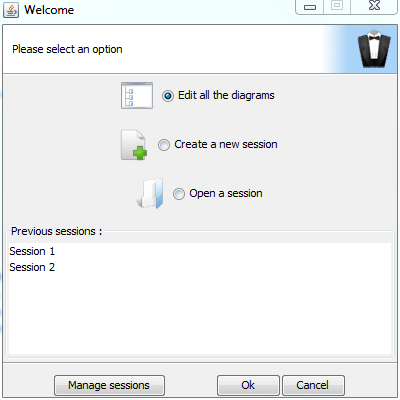
\includegraphics[scale=0.55]{images/ouverture_session.png}

\caption{L'assistant de choix de la session}
\end{figure}

\section{Création d'une nouvelle session}
La première chose à faire lors de la création d'une session est de nommer cette dernière. Cela se fait à l'aide du cadre "Nom de la session".\\

Ensuite, il faut ajouter les acteurs concernés. Pour cela, il faut sélectionner un acteur dans l'arborescence située sur la gauche de la fenêtre puis cliquer sur un des boutons "Ajouter un acteur principal" ou "Ajouter un acteur secondaire". Il est toujours possible par la suite de changer le type d'un acteur sélectionné.\\

Lorsqu'un acteur a ainsi été ajouté, il apparaît dans la liste correspondante ("Acteurs principaux" ou "Acteurs secondaires"). Chaque ligne correspond à un acteur. Il est possible :\\
\begin{itemize}
\item de supprimer l'acteur de la liste (petite croix juste avant le nom)
\item de renommer cet acteur pour la session
\item d'accéder à sa fiche (voir paragraphe \ref{fiche_acteur})
\item de changer le type de l'acteur (principal ou secondaire)\\
\end{itemize}



\begin{figure}[h!t]
\centering
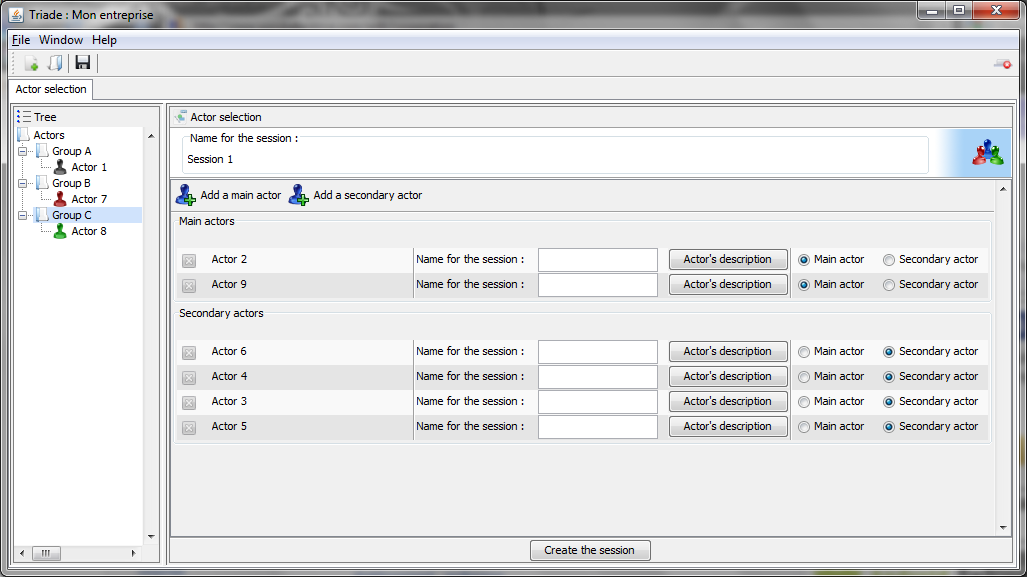
\includegraphics[scale=0.35]{images/selection_acteurs.png}

\caption{Création d'une nouvelle session, sélection des acteurs}

\end{figure}

Une fois la liste finalisée, il suffit de cliquer sur le bouton correspondant en bas de la fenêtre pour créer la session. Attention, il n'est plus possible de modifier la liste des acteurs une fois la session créée.\\

\section{Fiches des acteurs}
\label{fiche_acteur}
Chaque acteur est associé à une fiche. Elle permet de saisir les deux récits et de changer le nom associé à l'acteur. Chaque fiche est liée à une seule session (les récits saisis dans une session ne seront pas accessible depuis une autre). De plus un résumé de la situation de l'acteur est disponible à la suite des zones de texte.\\

Il est possible de revenir au nom par défaut d'un acteur en supprimant complètement le texte dans le champ "Nom associé à l'acteur "..." pour la session".\\

Les zones de textes "Premier récit", "Deuxième récit" et "Notes" permettent de saisir des informations concernant cet acteur.\\

La partie suivante présente un résumé de la situation de l'acteur, en triant les briques en fonctions des relations qui concernent cet acteur. En premier sont placés les briques présentant au moins une relation en écart, puis au moins une relation incomplète, et enfin celles n'ayant que des relations en accord. Il est possible d'accéder directement à une brique en cliquant sur son nom.\\

\begin{figure}[h!t]
\centering

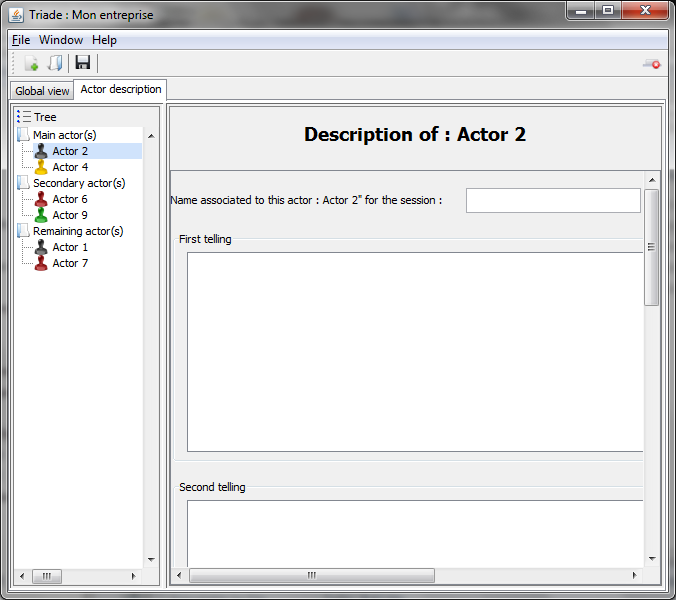
\includegraphics[width=12cm]{images/fiche_acteur.png}

\caption{La fiche d'un acteur}

\end{figure}

Il possible d'accéder à la fiche d'un acteur en faisant un clic droit sur ce dernier. Cela peut être fait dans un arbre ou dans une brique (voir figure~\ref{menu_fiche_acteur}). De plus l'arbre présent sur la gauche de la fiche d'un acteur permet d'accéder rapidement à l'ensemble des acteurs présent dans la sessions. La catégorie acteur restant correspond aux acteurs présent dans une brique mais n'ayant pas été sélectionné par l'utilisateur. Ces acteurs ne sont disponibles qu'une fois la session créée.\\

L'onglet "Liste des acteurs" permet à tout moment de retourner à l'affichage des fiches des acteurs.


\begin{figure}[h!t]
\centering
\Ovalbox{
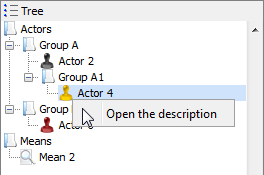
\includegraphics[width=6cm]{images/menu_fiche_acteur.png}
}

\caption{Le menu contextuel permettant d'ouvrir la fiche d'un acteur}

\label{menu_fiche_acteur}
\end{figure}

\section{Interface de gestion des sessions}
Cette interface est accessible depuis l'écran d'acceuil de \tria. Elle permet de gérer l'ensemble des sessions courantes. Les actions possibles sont :\\
\begin{itemize}
\item \textbf{Ouvrir} : Permet d'ouvrir la session sélectionnée. Si plusieurs sessions sont sélectionnées, un message d'erreur apparaît.\\
\item \textbf{Archiver} : Permet d'archiver des sessions dans un fichier. Ces sessions sont ensuite supprimées de la liste des sessions courantes.\\
\item \textbf{Sauvegarder sous} : Permet d'enregistrer une copie des sessions sélectionnées dans un fichier. Ces sessions sont conservées dans la liste des sessions courantes.\\
\item \textbf{Importer} : Permet d'ajouter à la liste des sessions courantes les sessions d'un fichier. Si une session portant le même nom qu'une session importée est déjà présente dans la liste, il sera demandé à l'utilisateur s'il veut remplacer la session présente dans la liste. Attention, en cas de remplacement, cette session sera perdue.\\
\item \textbf{Renommer} : Permet de renommer les sessions sélectionnées. Il est possible de renommer plusieurs sessions à la suite en faisant une sélection multiple.\\
\item \textbf{Supprimer} : Permet de supprimer des sessions. Attention, cette opération est irréversible.\\
\end{itemize}

Il est possible de sélectionner plusieurs sessions en même temps afin d'exporter dans un même fichier un ensemble de sessions. Pour cela la touche \textit{Ctrl} permet d'ajouter un élément à la sélection, et \textit{Maj} permet de sélectionner un groupe de sessions.\\

\begin{figure}[h!]
\centering
\Ovalbox{
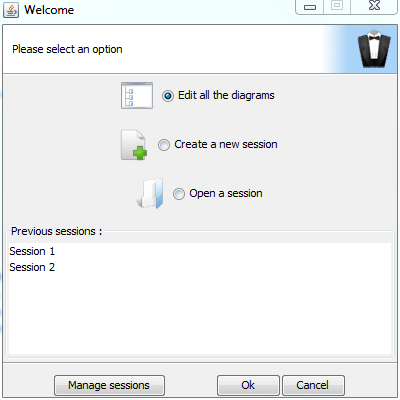
\includegraphics[width=0.6\textwidth]{images/ouverture_session.png}
}
\caption{L'interface de gestion des sessions\\est accesible depuis l'assistant d'ouverture}

\end{figure}
~
\begin{figure}[h!]
\centering
\Ovalbox{
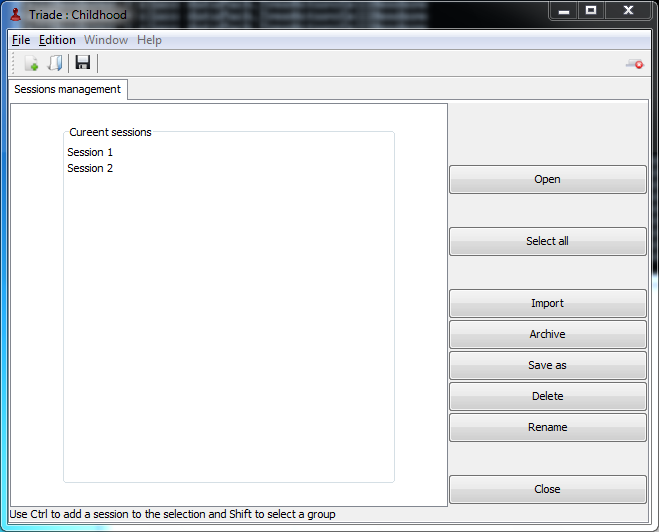
\includegraphics[width=0.8\textwidth]{images/gestion_session.png}
}
\caption{L'interface de gestion des session}
\end{figure}

% 2 Etapes et briques
% 2.1 Vue globale
% 2.2 Ouverture d'une brique
% 2.3 Edition des relations
\chapter{Bricks exploration}

% 2 Etapes et briques
% 2.1 Vue globale
% 2.2 Ouverture d'une brique
% 2.3 Edition des relations

After session creation, the user can access to all brick which contains the selected actors.\\
%Une fois la session créée, l'utilisateur peut accéder à l'ensemble des briques qui font intervenir les acteurs qu'il a sélectionnés.\\

The bricks are sorted by step.\\
%Les différentes briques sont regroupées par étape. Les étapes correspondent aux différentes phases du cas étudié.\\

\section{Global view}

Each step is associated to a global view. It's a presentation of the different bricks. The tree on the left present one folder by step. This folder contains all the bricks of the step and a folder for all the export of those bricks.\\
%Lors de l'ouverture ou de la création d'une session, une interface présentant les différentes vues globales apparaît. Chaque vue globale présente les briques d'une étape (il y a une vue globale par étape qui contient au moins une brique). L'arborescence sur la gauche de la fenêtre présente un dossier par étape, chacun d'eux contenant les briques de l'étape et les exports de ces briques (voir partie \ref{export}).\\

%Pour accéder à la vue globale, il suffit de cliquer sur son onglet ("Vue globale"). 

\begin{figure}[h!]
\centering

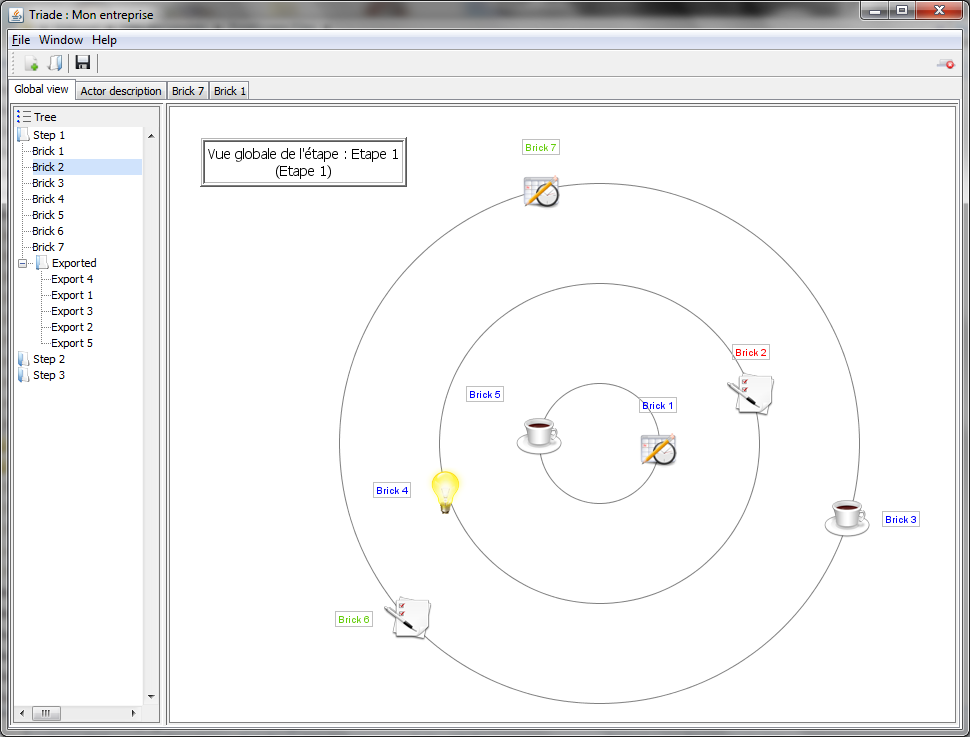
\includegraphics[scale=0.35]{images/vue_globale.png}
\caption{Global view of a step}

\end{figure}

The brick are displayed in three circle in the global view, the closer the bricks is from the center, the more important the role of selected actors is.\\
%Chaque vue globale se présente sous la forme de 3 cercles concentriques. Les briques sont disposés en fonction de l'importance des acteurs sélectionnés par l'utilisateur dans ces briques.
%\begin{itemize}
%\item Dans les briques les plus au centre, les acteurs principaux de l'utilisateur ont un rôle central.
%\item Dans le deuxième cercle, les acteurs principaux ont un rôle secondaire et/ou les acteurs secondaires ont un rôle central ou secondaire.
%\item Dans le troisième cercle les acteurs sélectionnés ont un rôle peu important.\\
%\end{itemize}

The color of brick labels show the state of the relations of the brick :\\
%La couleur des étiquettes des différentes briques indique si les relations de ces briques ont été remplies ou non, et si elles sont en écart. 
\begin{itemize}
\item Blue for incomplete relation.
%\item Le bleu correspond à une brique où des relations n'ont pas été remplies.
\item Red for gapped relation.
%\item Le rouge correspond à une brique où au moins une des relations est en écart.
\item Green for correct relation.\\
%\item Le vert correspond à une brique où toutes les relations sont remplies et aucune ne présente d'écart.
\end{itemize}

If a brick contains incomplete and gapped relation, its label will be blue.\\
%Le rouge étant prioritaire sur le bleu, une brique comportant des relations pas encore remplies et au moins une relation en écart apparaîtra en rouge.\\

You can access to all the exports of a brick by making a right click on his name, or in an empty space in the scheme.\\
%Il est possible d'accéder d'accéder à toutes les exportations réalisée sur une brique en faisant un clic droit sur cette dernière (voir le chapitre \ref{export} sur les exportations).\\

To open a brick, just do a double click on it in the tree or in the global view.\\
%Pour ouvrir une brique, il suffit de faire un double-clic sur son icône dans une vue globale ou sur la ligne de l'arbre correspondante. Un nouvel onglet apparaĩt  pour afficher cette brique. Plusieurs briques peuvent être ouverte en même temps. 

\section{Bricks and relation}
Each brick represent a possible real situation. The different component of the scheme represent the actors, the tools and the activity of the situation.\\
%Chaque brique représente une situation qu'il est possible de rencontrer dans la réalité. Les différents éléments du schéma représente les acteurs, les moyens et l'activité qui composent la brique.\\

\begin{figure}[h!]
\centering
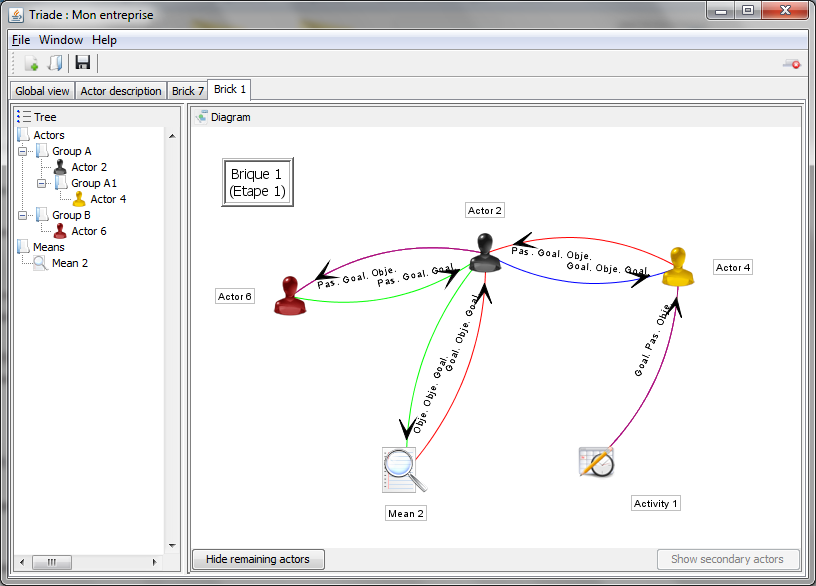
\includegraphics[scale=0.55]{images/brique.png}
\caption{A brick view}

\label{brique}
\end{figure}
When you open a brick for the first time, only the main actors are showned. You have to use the two buttons on the bottom of the window to show more or less actors.\\
%Les éléments apparaissent progressivement afin de permettre à l'utilisateur d'assimiler les différents éléments de la situation. Les deux boutons situés en dessous du schéma permettent d'afficher et de masquer les éléments de la brique.\\

%Les éléments apparaissent dans l'ordre suivant :\\
%\begin{enumerate}
%\item Les moyens, les activités, les acteurs principaux et ceux ayant un rôle central dans la brique.
%\item Les acteurs secondaires et ceux ayant un rôle secondaire.
%\item Les acteurs restants.\\
%\end{enumerate}

A relation between two actors is represented by an arrow from the first actor to the second. The return relation is represented by an opposite arrow (from the second to the first). Those arrow will be sometime called "edge" in this manual.\\
%Les relations entre deux acteurs sont représentées par des flèches entre deux éléments d'un schéma. Ces flèche sont orientées, ainsi une flèche allant d'un acteur A vers un acteur B représente la relation que A a envers B, la relation retour (ie. de B vers A) est associée à la flèche retour.\\

There are two way to select an edge, by clicking on it (or on its label), or by dragging the mouse (while cliking) from the first actor to the second.\\
%Deux manières permettent de sélectionner une arête. Soit en cliquant dessus (ou sur son étiquette), soit en faisant un clic continu à partir du premier acteur jusqu'au deuxième.\\

\begin{figure}[h!]
\centering
\Ovalbox{
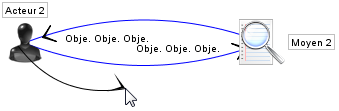
\includegraphics[height=25pt]{images/selection_1.png}
}
\Ovalbox{
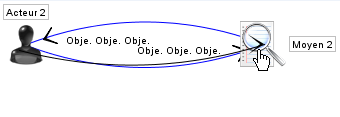
\includegraphics[height=25pt]{images/selection_2.png}
}
\Ovalbox{
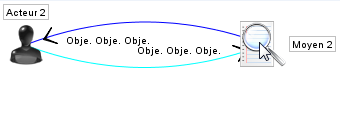
\includegraphics[height=25pt]{images/selection_3.png}
}
\caption{A edge selection by dragging}

\end{figure}

When a relation is selected, a pop-up appears. It allow the user to consult the relation and to fill and modify the real relation. The goals and the meanings for action time could be selection in a list of possibility. The structural relation is showned but it can't be modified.\\
%Lorsqu'on sélectionne une relation, une fenêtre apparaît. Elle permet de consulter et modifier la relation. Il est possible de définir les objectifs et les moyens réels de chaque temps d'action. Une liste de possibilité est fournie pour chaque champ. La relation structurelle est affichée dans cette fenêtre mais ne peut pas être modifiée.\\

The content of an action time could be copied in the next action time by clicking with the button with a down arrow on the left of the line.\\
%La petite flèche située sur la gauche d'un objectif permet de répliquer l'objectif et le moyen réel au temps d'action suivant.

\begin{figure}[h!]
\centering
\Ovalbox{
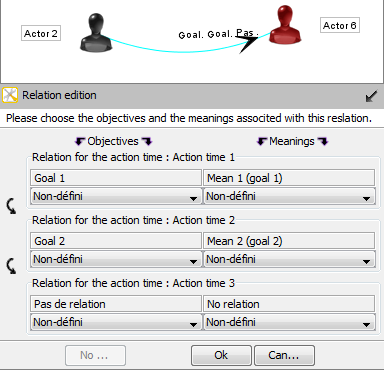
\includegraphics[scale=0.75]{images/edition_relation.png}
}
\caption{Relation edition pop-up}
\label{edition_relation}
\end{figure}

The color of the edge show if the relation is incomplete (blue), gapped (purple for a gap on meanings, red for a gap on goals) or correct (green).\\
%Les relations apparaissent d'une couleur différente en fonction de leur état. Le code couleur utilisé est le même que celui des briques (voir figure~\ref{brique} pour les couleurs des arêtes) :
%\begin{itemize}
%\item Bleu pour une relation incomplète (certains objectifs sont encore à "Non-défini").
%\item Rouge foncé pour une relation en écart au niveau d'un moyen (un des moyens réels est différents du moyen structurel mais les objectifs sont tous en accords).
%\item Rouge clair pour une relation en écart au niveau d'un objectif (un des objectifs réels est en écart, le moyen n'est pas pris en compte).
%\item Vert pour une relation réelle en accord avec la relation structurelle (tous les objectifs et les moyens concordent).
%\end{itemize}

Don't forget to display all actors (with the two buttons on the bottom of the window) in order to see all the relations.\\
%Attention, n'oubliez pas de faire apparaître l'ensemble des acteurs pour avoir accès à toutes les relations d'une brique.\\

Relations are associated to tool-tip which describe entirely the relations. You just have to let the mouse pointer over an edge during 1 second to show the tool-tip.\\
%Les relations sont associées à des info-bulles qui fournissent un résumé complet des objectifs et des moyens de la relation. Il suffit de placer la souris sur une flèche pendant une seconde pour faire apparaître l'info-bulle.\\

It is possible to add an absent relation. But all the structural goals and meanings will be set to "No relation", If the user set all the real relation to "No relation", the edge won't be shown.\\
%Il est possible d'ajouter une relation absente. Cependant, tous les objectifs structurels seront mis à "Pas de relation", de ce fait cette relation sera forcément en écart. Si l'utilisateur définit tous les objectifs réels à "Pas de relation", l'arête ne sera pas affichée.\\

%L'arborescence sur la gauche de la fenêtre présente l'ensemble des acteurs présents dans la brique. Elle permet de sélectionner rapidement un acteur et aussi d'accéder à sa fiche à l'aide d'un clic droit.\\

You can move a vertex with pressing "Shift" in while dragging the vertex. With "Ctrl" you can move the whole scheme.\\
%Il est possible de déplacer un sommet en maintenant la touche "Ctrl" appuyée tout en cliquant sur le sommet. De même pour déplacer l'ensemble des sommets, il faut cliquer sur la touche "Majuscule" (shift) tout en cliquant.\\ 



\section{Default edge label}
It is possible to change the default edge label content. The sub-menu "Brick edge labels" allow the following possibilities : 
%Il est possible de changer le contenu par défaut des étiquettes des arêtes dans les briques. Le sous-menu "Etiquettes des arêtes des briques" dans le menu Edition. Les   différents contenus sont :\\
\begin{itemize}
\item \textbf{Structural relations} : Display the 4 first characters of structural relations for each action times.\\
%\item \textbf{Relations structurelles} : Affiche les 4 premiers caractères des relations structurelles de chaque temps d'action.\\
\item \textbf{Real relations} : The same with real relations.\\
%\item \textbf{Relations réelles} : De même avec les relations réelles.\\
\item \textbf{Relation at action time : *} : Display the structural and the real relations for the selected action time.\\
%\item \textbf{Relation au temps d'action : *} : Affiche la relation structurelle et la relations réelle pour le temps d'action sélectionné.\\ 
\end{itemize}

This setting affect only the edge labels in the bricks. In the exports, edge labels are controlled by the global export settings (see also section \ref{globalExport}).\\
%Cette option ne concerne que les relations dans les briques. Dans les exports, ces étiquettes sont contrôlées par les options globale de l'export (voir paragraphe \ref{globalExport}).\\

\begin{figure}[h!]
\centering
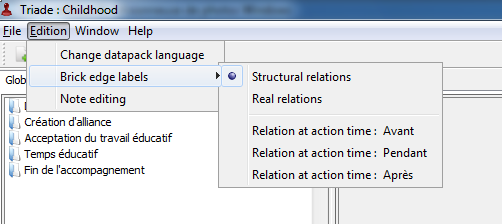
\includegraphics[width=0.5\textwidth]{images/menu_edition.png}
\caption{The default edge label sub-menu}
\label{menu_edition}
\end{figure}


\section{Note editing in bricks}
Each brick is associated with a note. It is useful to keep information and to add some explanation for the situation described in the brick. By default, note are not editable. The option "Note editing" have to be selected to enable note editing. This option is in the edition menu (see picture \ref{menu_edition}). A note is associated to a session, it will be only accessible from the session in which it has been created.\\
%Chaque brique est maintenant associée à une note. Cela permet d'ajouter des informations pour décrire une situation. Par défaut, les notes ne sont pas éditables. Il faut activer l'option "Edition des notes" dans le menu édition avant de pouvoir les modifier (voir image \ref{menu_edition}).\\

Notes are displayed in the upper-right corner of the brick window. The note could be hidden or displayed by clicking on the arrow.\\
%Les notes sont accessibles à l'aide du cadre présent en haut à droite de la zone d'affichage d'une brique. Attention, les notes sont liés à une brique et à une session. En particulier, elles ne sont pas partagées entre les sessions.\\

\begin{figure}[h!]
\centering
\begin{subfigure}{\textwidth}

\centering
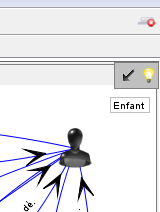
\includegraphics[width=0.4\textwidth]{images/note_fermee.png}
\caption{A note in hidden mode}
\end{subfigure}
\begin{subfigure}{\textwidth}

\centering
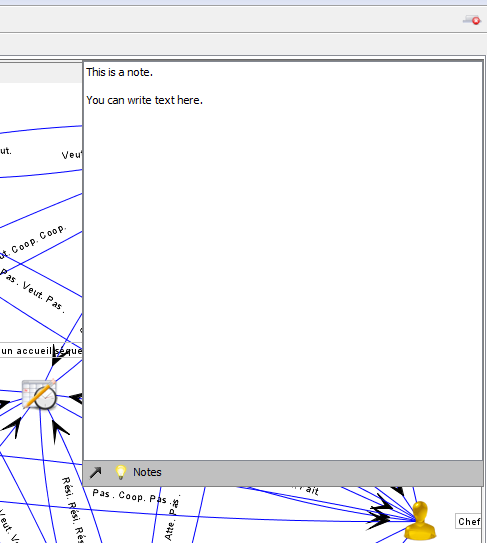
\includegraphics[width=0.4\textwidth]{images/note_ouverte_edition.png}
\caption{An opened note with editing mode enabled}
\end{subfigure}
\begin{subfigure}{\textwidth}

\centering
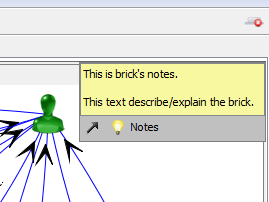
\includegraphics[width=0.4\textwidth]{images/note_ouverte_pas_edition.png}
\caption{An openend note with editing mode disabled}
\end{subfigure}

\end{figure}




% 3 Export vers des images
% 3.1 Element modifiables
% 3.2 Ajout d'images personnelles
% 3.3 Génération d'images
\chapter{Les exports}
\label{export}

Une fois les briques remplies et les lieux de problème identifiés, il est possible de générer des images des schémas porteurs d'informations. De plus, il est possible de personnalisé l'apparence de ces schémas pour les adapter au type de diffusion.\\

Un export correspond à la personnalisation d'un schéma en vue de la génération d'une image.\\


\begin{figure}[h!t]
\centering
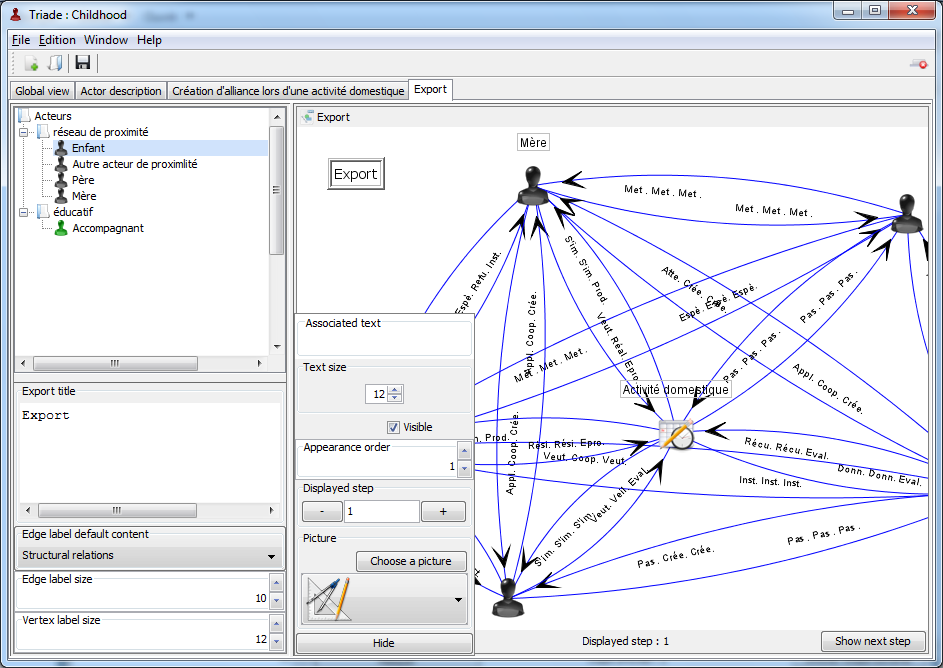
\includegraphics[scale=0.45]{images/vue_export.png}

\caption{Un schéma en cours de personnalisation.}

\end{figure}


\section{Création et accès à un export}

Il existe plusieurs manières de créer un export d'un schéma :\\
\begin{itemize}
\item Depuis une vue globale en faisant un clic droit sur une des briques. Un menu apparaît et permet de créer un nouvel export et d'accéder à tous les export réalisé sur cette brique dans cette session.\\
\item Depuis la vue d'une brique, un clic droit sur le schéma au dessus d'aucun sommet fait apparaître le même menu. Un clic droit sur un des sommets permettra d'accéder à la fiche acteur de ce sommet.\\
\item A l'aide du dossier "exportés" présent dans chaque dossier d'étape dans l'arborescence sur la gauche des vues globales.\\
\end{itemize}
 
Lors de la création d'un export, une boite de dialogue vous invite à saisir le nom qui sera donné à cet export. Il apparaîtra dans un cadre en haut à gauche de l'image générée.\\


\begin{figure}[h!]
\centering
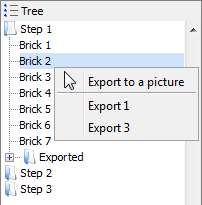
\includegraphics[scale=0.75]{images/menu_export.png}
\caption{Le menu contextuel d'accés et de création des exports.}
\end{figure}

Il est possible de supprimer un export depuis la vue globale en faisant un clic droit sur l'export à supprimer. Attention, l'export ne disparaîtra de la liste des exports que lors du lancement suivant du logiciel. 

\section{Personnaliser l'apparence d'un schéma}

De nombreux éléments peuvent être personnalisés dans le cadre d'un export :\\
\begin{itemize}
\item La position des sommets
\item Le texte associé à un sommet (acteur, moyen ou activité) ou à une relation.
\item La taille de ces textes
\item La couleur d'une arête
\item L'image utilisée pour représenter un sommet
\item La visibilité d'un sommet ou d'une arête
\item L'ordre d'apparition des éléments\\
\end{itemize}
\begin{figure}[h!]
\centering
\subfloat[Pour un sommet]{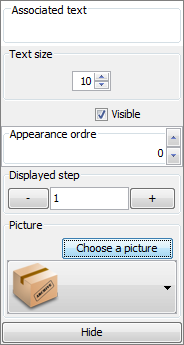
\includegraphics[height=9cm]{images/export_vertex.png}}
\hspace*{35pt}
\subfloat[Pour une relation]{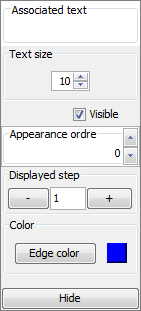
\includegraphics[height=9cm]{images/export_edge.png}}

\caption{Les pop-up de personnalisation}
\label{popup}
\end{figure}

Il suffit de sélectionner un sommet ou une arête pour faire apparaître le module de personnalisation de cet élément.\\

\subsection{Déplacement d'un sommet}
Pour déplacer un sommet, il suffit d'appuyer sur la touche "Majuscule" (shift) tout en réalisant un clic continu sur le sommet.\\

\subsection{Modification des étiquettes}

Le champ "Texte associé" permet de modifier l'étiquette d'un sommet ou d'une arête. Pour retrouver le texte initial, il suffit d'effacer complètement le texte saisi. Pour n'afficher aucune étiquette il est possible de ne mettre qu'un espace dans le champ.\\

La modification de la taille du texte d'une étiquette se fait à l'aide du champ "Taille du texte". La valeur par défaut est 10.\\

\subsection{Couleur des arêtes}

Il est possible de choisir la couleur d'une arête avec le bouton correspondant. \\

\subsection{Image d'un sommet}
Il est possible de changer les images de chaque sommet. La zone Image contient une liste et un bouton "Choisir une image" à cet effet.\\



La liste permet d'accéder aux dernières images utilisées. Il suffit de cliquer sur une image pour l'associer au sommet. Le bouton permet d'ouvrir une fenêtre donnant accès à toutes les images disponibles. Sont proposées en premier les images internes à \tria.\\



Il est possible de cocher la case "Appliquer l'image a toute la session" pour utiliser cette image pour ce sommet dans tous les exports de cette session. Pour annuler ce choix, il suffit de choisir l'image que le sommet avait initialement comme image par défaut.\\ 

\begin{figure}[h!]
\centering
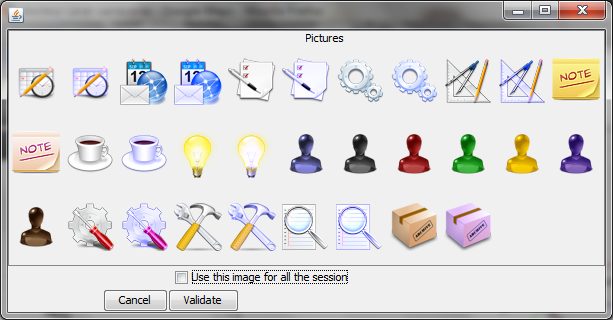
\includegraphics[scale=0.65]{images/choix_image.png}
\caption{La fenêtre de choix de l'image d'un sommet.}
\end{figure}

 Vous pouvez ajoutez vos propres images en les copiant dans le dossier "Triade/pics" qui se situe dans votre dossier personnel. Ces images seront automatiquement redimensionnée et le blanc sera passé en couleur transparente.\\


\subsection{Visibilité des éléments}
La case à cocher "Visible" permet de masquer un sommet ou une arête. Attention, lorsqu'un sommet ou une arête ont été masqués, il n'est plus possible de les sélectionner en cliquant dessus. Il faut passer par l'arborescence sur la gauche pour sélectionner un sommet masqué (un suffixe (caché) est ajouté au nom du sommet). Pour une arête, il faut faire un clic continu à partir du premier jusqu'au deuxième sommet de la relation.\\

Les arêtes aboutissant à un sommet masqué ne sont jamais affichées.\\



\subsection{Ordre d'apparition des éléments}

Afin de présenter plus facilement une situation à des interlocuteurs extérieurs, il peut être utile de faire apparaître progressivement les éléments d'un schéma. L'ordre d'apparition sert à cela.\\

Chaque élément (sommet ou arête) est associé à un ordre d'apparition. Il permet déterminer à partir de quand l'élément sera affiché. Par exemple, un sommet ayant un ordre d'apparition à 2 apparaîtra à l'étape 2, 3, etc... mais pas à l'étape 1.\\

Le bloc "Etape affichée" permet de contrôler l'étape actuellement affichée dans le schéma. Il est possible de changer l'étape à l'aide des deux boutons situés au dessous du schéma ou à l'aide du menu contextuel qui s'ouvre sur l'ensemble du schéma (clic droit).\\

Attention, si vous mettez un ordre d'apparition supérieur à l'étape courante, le sommet concerné disparaîtra. Il n'apparaîtra que aux étapes supérieurs à son ordre d'apparition.\\

Le nombre d'étape dépend du plus grand ordre d'apparition d'un élément du schéma. L'ordre d'apparition maximal étant 25.\\

Lors de la génération de l'image, une image par étape utile sera générée. Une étape utile contient au moins un élément apparaissant à cette étape.\\

\section{Options globales lors d'un export}
\label{globalExport}
Le cadre présent sous l'arbre des acteurs sur la gauche de la fenêtre permet de contrôler plusieurs éléments portant sur l'ensemble de l'export.\\

Le premier champ permet de modifier le titre de l'export. Laisser ce champ vide masque le cadre de titre.\\

Le champ suivant permet de modifier les étiquettes par défaut des arêtes. Il est possible de masquer l'ensemble des arêtes avec l'option "Aucune étiquette". Cela permet de n'afficher que les étiquettes des arêtes modifiées manuellement.\\

Les deux champs suivants permettent de modifier la taille par défaut des étiquettes des sommets et des arêtes.\\

\begin{figure}[h!]
\centering
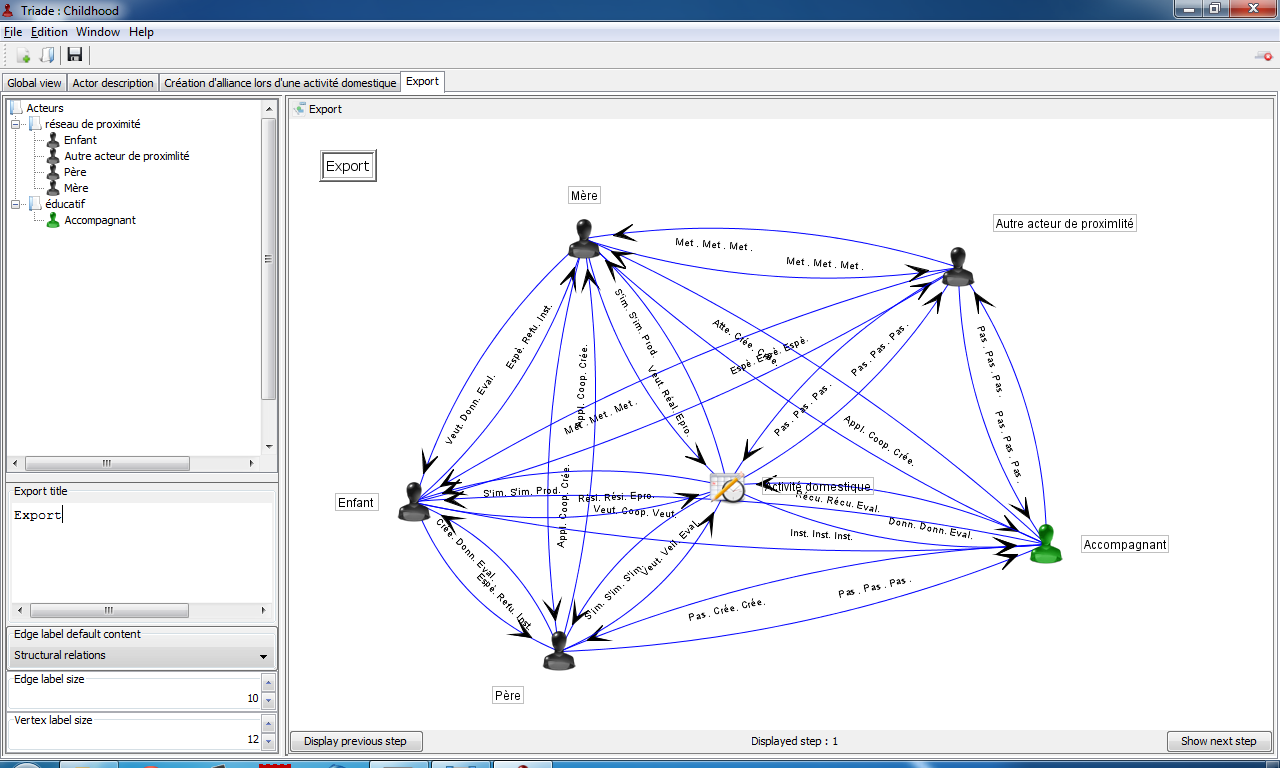
\includegraphics[width=0.5\textwidth]{images/export_global.png}
\caption{Ces options se règlent à l'aide du cadre en bas à gauche de la fenêtre}
\end{figure}


\section{Générer une image}

Une fois la personnalisation de l'export terminé, il est nécessaire de générer l'image. Il suffit pour cela de faire un clic droit sur le schéma. La première option du menu contextuel est "Générer une image".\\

Une fenêtre s'affiche afin de laisser l'utilisateur choisir à quel endroit l'image sera enregistrée. Si aucune extension n'est ajoutée, l'image générée sera au format PNG. Il est cependant possible d'ajouter l'extension de son choix (jpg, png, gif) pour changer de format d'image.\\

Si l'export contient plusieurs étapes d'apparition, plusieurs fichiers seront générés. Le nom fourni par l'utlisateur sera préfixé par "\_Etape\_1" pour la première étape et ainsi de suite.\\

\begin{figure}[h!]
\centering
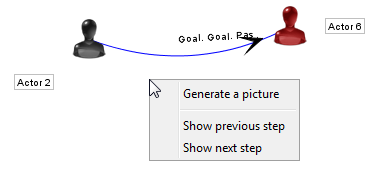
\includegraphics[width=6cm]{images/generer_image.png}

\caption{Le menu de génération d'une image}

\end{figure}

  




% 4. Système d'envoi de mail
% 4.1 Demande d'ajout d'une relation
% 4.2 Rapport d'erreur

\chapter{Mail sending system}

Two kind of mail can be sent in \tria :
%Un module du programme permet d'envoyer des mails au créateur de l'ensemble des schémas et au développeurs de l'application. Deux types de mails peuvent être envoyés :\\
\begin{itemize}
\item A request to add a new relation.\\
%\item Une demande d'ajout d'une nouvelle relation. 
\item A report when an error has been met.\\
%\item Un rapport lorsqu'une erreur est survenue dans le logiciel. 
\end{itemize}

\section{Relation adding request}
In certain situations, it possible that the user do not find the real relation he needs. The objective "Other" is the first solutions to this kind of problem. But if the same relations is often needed, it possible to ask the schemes creator to add the relations to the lists of possibility in the next update.\\
%Dans certains, il est possible que l'utilisateur ne trouve pas de relation réelle convenant à la situation qu'il rencontre. L'objectif "Autre" permet de répondre à ce problème. Cependant, si une même relation manque à de nombreuses reprises, il est intéressant d'en informer le créateur de l'ensemble de schémas afin qu'il l'intègre à une futur version.\\

To do so, just lick on the option "Relation adding request" in the menu "Help".\\
%Pour réaliser cette demande, il suffit de cliquer sur l'option "Demande d'ajout de relation" dans le menu "Aide". Une fenêtre s'ouvre alors.\\


%L'adresse de réponse permet au destinataire de vous répondre directement.\\

%Les deux champs suivants correspondent au sujet et au contenu du mail envoyé.\\


\begin{figure}
\centering
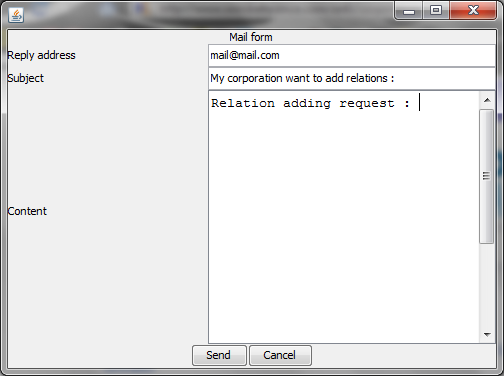
\includegraphics[width=12cm]{images/mail_relation.png}
\caption{The relation adding request window.}
\end{figure}


\section{Error report}

In despite of all the test realized in order to distribute a software of quality, it is still possible than some errors exist. If an error occurs, a pop-up will show and ask the user to send an error report. If this error is met for the first time, it is important to send this report with a description as precise as possible of the context of the error.\\ 
%Malgré l'ensemble des tests réalisés sur le logiciel \tria, il est possible qu'il subsiste quelques problèmes. Dans le cas où une erreur est rencontré, le logiciel vous propose automatiquement d'envoyer un mail aux développeurs. Cela leur permet d'identifier l'erreur et de la corriger par la suite.\\

%Il est très important de décrire l'action que vous étiez en train de réalisez lorsque l'erreur s'est produite. Cette description est une information souvent indispensable à la résolution du problème. Un texte généré automatiquement à l'intention des développeurs est ajouté à la fin du mail.\\

%Une boite de dialogue informe l'utilisateur qu'il est plus prudent de quitter l'application. Si c'est une erreur encore inconnue, il est fortement conseillé de quitter l'application. Dans le cas d'une erreur bénigne, les développeurs informeront l'utilisateur qu'il peut tout de même continuer à travailler (en répondant par mail à l'envoi du rapport d'erreur).\\







% 5. StringTranslator
\chapter{Translations management}

\section{Translation module}
The software \tria is sold with a translation module in certain situation.\\
%Dans certain cas, le logiciel \tria est fourni avec un module de traduction.\\

Warning, it is not possible to use \tria and the translation module in the same time. You have to close the translation module to see the result in \tria.\\
%Attention, il n'est pas possible d'utiliser simultanément le module de traduction et \tria. Vous devez fermer le module de traduction pour voir le résultat dans \tria.\\

This module allow to translate every text which appear in the schemes set : \\
%Ce module permet de traduire les chaînes de caractères qui apparaissent dans un ensemble de schémas. Ces chaînes correspondent aux noms des éléments suivants :\\

\begin{itemize}
\item Actors
%\item Les acteurs
\item Bricks
%\item Les briques
\item Tools
%\item Les moyens
\item Activity %\item Les activités
\item Action times
%\item Les temps d'actions
\item Steps
%\item Les étapes
\item Objectives
%\item Les objectifs
\item Meanings\\
%\item Les moyens\\
\end{itemize}

The translation module works directly with the data file used in \tria. When a translation is associated to a text, it is automatically used in \tria.
%Le module de traduction travaille directement sur le fichier utilisé par \tria. Lorsqu'une traduction est associée à une chaîne de caractère, elle sera utilisée lors de l'utilisation suivante de \tria.

A filter field is avaible in the top of the window. The filter is applied on the translation and the original text.\\
%Un champ de recherche permet de filtrer les entrées affichées dans la fenêtre. La recherche est effectuée sur le terme initial et sa traduction.\\


%Pour utiliser le texte initial au lieu d'une traduction, il suffit d'effacer entièrement le texte de la traduction.\\
It is possible to get statistics about the translation with the button "Translation statistics" on the bottom left of the window.\\


\section{Datapack translation management}
It is possible to export and to import translation of the datapack. Use the corresponding buttons in the bottom of string translator interface \\
%Il possible d'importer et d'exporter une traduction depuis le module de traduction.\\

Warning, the current translation is lost when a new one is imported. Verify if you need to export before import the new one.\\
%Attention, lors d'une importation, la traduction est perdue. Veillez à exporter cette dernière avant si vous voulez la conserver.\\

It is also possible to change the translation from \tria with the option "Change datapack language" in the Edition menu (see picture \ref{menu_edition}). As in String translator module, the current translation will be lost.\\
%Il est aussi possible de changer la traduction depuis le datapack avec l'option "Changer la langue du datapack" dans le menu Edition (voir image \ref{menu_edition}). De même, la traduction actuelle sera écrasée lors de cette opération.\\


\begin{figure}[h!]
\centering
\Ovalbox{
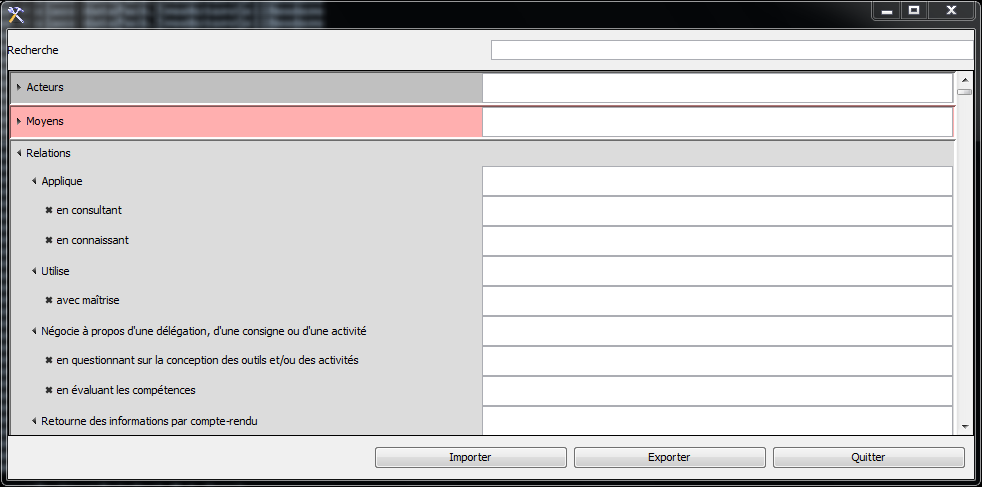
\includegraphics[width=0.8\textwidth]{images/translator.png}
}
\caption{The string translator interface.}
\end{figure}


\section{Selection of software interface language}
The language of software interface can be changed with the "Language" menu in the main window. The software needs to be restarted after a change of language.
%La langue de l'interface peut être choisie à l'aide du menu "Langue" dans l'interface principale. Le logiciel doit être redémarré après un changement de langue.\\

It is possible to add a new language by adding the corresponding file in the sub-folder "language" in the installation \tria folder. To do so, make a copy of any other language file, rename it with the correct code and translates every sentences in the file. The new language will be automatically added to the list of available language in the "Language" menu.\\
%Il est possible d'ajouter une nouvelle langue en ajoutant le fichier correspondant dans le sous dossier "language" du répertoire d'installation du logiciel. Pour réaliser cette traduction, il suffit de réaliser une copie d'un des fichier puis de traduire l'ensemble des phrases qu'il contient. La nouvelle langue sera proposée dans le menu "Langue" lors du démarrage suivant du logiciel.\\

If some sentences are not translated in the software, that could comes from missing sentences in the translation file. In this case, french translation is used instead. That could be corrected by adding the missing sentences in the corresponding file in the language folder.\\
%Si des phrases sont manquantes dans un fichier de traduction, celles de la version françaises seront automatiquement utilisées à la place. De ce fait, si certaines phrases sont en français, cela signifie sûrement que leur traduction est manquante. 





% 6. Fonction limitée à la version prof
% 6.1 génération de licence et de datapack
%
\chapter{Teachers version features}

The "Tools" menu, only available in the teacher version, allow user to generate use-licenses and limited time datapack for student version. 
%Le menu "Outils", uniquement présent dans la version enseignant du logiciel, permet de générer des licences d'utilisation ainsi que d'exporter des datapack à destination des versions étudiantes.

Those two tools request user to enter his personnal key. This key has been normally given to you during software distribution. If not, please contact developpers team.\\
%Lors de l'utilisation de ces deux outils, il vous est demandé de saisir votre clé personnelle. Cette dernière vous a normalement été fournie lors de la livraison du logiciel.\\

\section{Licenses generation}

The first step of licenses generation is to enter the list of mail address for which a license needs to be generated. This list could be extract from the clipboard, the mail address should be separated by ',' or ';' or a tabulation or a line jump. This function allow to import the list from a spreadsheet software.\\
%La génération de licences se déroule en deux étapes. Tout d'abord, l'utilisateur doit saisir la liste des adresses mails pour lesquelles une licence doit être générée. Il est possible d'extraire cette liste depuis le presse-papier. Dans ce cas, les séparateurs utilisés sont au choix : la virgule, le point-virgule, la tabulation et le retour chariot. Cela permet en particulier d'importer facilement cette liste depuis un tableur.\\

It is also possible to add an address with the dedicated field and button in the top of the window. Entries can be modified or deleted with the button on the top right of the window.\\
%Il est aussi possible d'ajouter une adresse à l'aide du champ mail et du bouton juste à sa droite situé en haut de la fenêtre. Les différentes entrées pouvant être modifiées et supprimées à l'aide des boutons dédiés en haut à droite de la fenêtre.\\

License type could be selected with the radio-button list on the bottom of the window. It is not possible to specify different licence for a same list. The option "Already billed licenses" allow to regenerate an unlock key for an user who have lost his key.\\
%Le type de licence peut être choisi à l'aide de la liste à puce en bas de la fenêtre. Il n'est pas possible de spécifier plusieurs licences différentes pour une même liste. L'option "Licence déjà facturée" permet de générer à nouveau un code de licence au cas ou ce dernier aurait été perdu par l'utilisateur.\\

The next step is to generate licences. Warning, an internet connection is requested during this step. The process is launched with the button "Generate licences" in the bottom right of the window. The mail list won't be editable further.\\
%L'étape suivante consiste à générer les licences. Attention, un connexion internet sera nécessaire lors de cette étape. Le processus est lancé lors du clic sur le bouton "Générer les licences". La liste de mail ne sera plus modifiable par la suite.\\

The user have to select the file which a summary of all generated licenses have to be saved. Then , it is possible to copy a mail address, an unlock key, a couple mail/key or the while list with the buttons on the right of the window.\\
%L'utilisateur est invité à choisir le lieu d'enregistrement du fichier de licence dans lequel il veut stocker le récapitulatif des licences générés. Il est ensuite possible de copier au choix une adresse mail, un code de déblocage, un couple mail/code de déblocage ou la liste entière à l'aide des boutons situés sur la droite de la fenêtre.\\

Once the window has been closed, it is not possible to access to the generated key list in the software, but only by the summary file saved during the process.\\
%Une fois la fenêtre de génération des licences fermées, il n'est plus possible d'accéder à la liste générées au sein du logiciel, mais uniquement grâce au fichier récapitulatif créé lors de la génération.\\


A billing request will be automatically send to the software dealer during licenses generations.\\
%Une demande de facturation est automatiquement envoyé à l'équipe de développement lors de la génération des licences.


\section{Generation of limited time datapack for student version}%Génération d'un datapack pour les version étudiantes}

The other option of tools menu allow to generate trial datapack. In this purpose, the user has to enter the trial period duration. The maximum is 365 days, and the minimum is 0. The trial period start on the datapack generation day. If the value 0 is used, the datapack will be always locked. It is usefull for user who had bought a license and who needs to reinstall the software. They can download a datapack of this kind and then unlock it whit their license key.\\
%L'autre option du menu outils permet de générer des datapack pour les versions étudiantes du logiciel. Lors de cette opération, l'utilisateur est tout d'abord invité à saisir la durée de validité du datapack. La durée maximale est de 365 jours. La durée minimale est 0 jours, cela correspond à un datapack bloqué immédiatement. Ce type de datapack est destiné à être mis à disposition des utilisateurs ayant acheté une licence d'utilisation afin qu'(il puisse le télécharger lors d'une réinstallation ultérieure du logiciel.\\

After setting the trial duration, the user have to select where to save the trial datapack. Then, the datapack will be automatically exported.\\
%La fenêtre suivante invite l'utilisateur à choisir l'endroit ou le datapack devra être enregistré.\\

%Une fois l'emplacement choisi, le datapack est automatiquement exporté.\\




\input{conclusion}


\end{document}
